\documentclass[12pt]{article}
\usepackage{geometry}
\geometry{
	left=20mm,
	top=20mm,
}
\usepackage[utf8]{inputenc}
\usepackage[shortlabels]{enumitem}
\usepackage{array}
\newcolumntype{C}[1]{>{\centering\let\newline\\\arraybackslash\hspace{0pt}}m{#1}}
\usepackage[spanish,es-nodecimaldot]{babel}
 \usepackage{url}
\usepackage[spanish, fixlanguage]{babelbib}
\bibliographystyle{IEEEtran}
\usepackage{graphicx}
\graphicspath{ {./images/} }
\usepackage{amssymb}
\usepackage{amsmath}
\usepackage{subcaption}
\usepackage[linesnumbered]{algorithm2e}
\newcommand\mycommfont[1]{\footnotesize\ttfamily\textcolor{blue}{#1}}
\SetCommentSty{mycommfont}
\usepackage{tikz}
\usetikzlibrary{positioning, fit}
\usetikzlibrary{babel}
\usepackage{titlesec}
\titlespacing*{\section}
{0pt}{5.5ex plus 1ex minus .2ex}{.3ex plus .1ex}
\titlespacing*{\subsection}
{0pt}{5.5ex plus 1ex minus .2ex}{2.3ex plus .1ex}
\title{Tarea 1: Recordatorio de Probabilidad}

\author{
	Saul Ivan Rivas Vega \\
	\\
	Aprendizaje Automatizado\\
}

\date{\today}

\begin{document}
	\maketitle
	\pagebreak
	\section{Ejercicio 1.}
	  \paragraph{} Se usa el siguiente proceso aleatorio para meter 2 pelotas en una caja: se tira una moneda y
	  se mete una pelota roja si sale águila o azul si sale sol. Posteriormente de esta caja se sacan
	  repetidamente de forma aleatoria con reemplazo 3 pelotas, las cuales resultan rojas. ¿Cuál es
	  la probabilidad de que las 2 pelotas de la caja sean rojas?.
	  \\
	  \paragraph{Solución: } Dado que al sacar 3 pelotas con reemplazo y que fueron rojas podemos decir que en la caja no hay dos pelotas azules. Solo es posible que haya 2 pelotas rojas o 1 roja y 1 azul.
	  \\
	  Inicialmente para meter la primera pelota a la caja tenemos 2 posibilidades, meter una pelota roja (Evento 1 $E_1$) o una azul (Evento 2 $E_2$).
	  Asumiendo que la moneda es justa, es decir que hay una misma probabilidad de que salga águila o que salga sol, la probabilidad de $E_1$ y $E_2$ es $0.5$ para ambas.
	  \begin{equation}
	  \begin{split}
	  	P(E_1)&=0.5\\
	  	P(E_2)&=0.5
	  \end{split}
	  \end{equation}
	  Ahora que sucede cuando revisamos las probabilidades de que la segunda pelota sea roja ($E_3$) o que sea azul ($E_4$) dado $E_1$ o $E_2$.\\
	  \paragraph{}\textbf{Si es que la primera pelota fue roja ($E_1$)}\\ 
	  $E_3$ requiere que la moneda caiga en águila lo cual asumimos ocurre con $0.5$ de probabilidad. Al ser independiente este evento de $E_1$ podemos calcular la probabilidad de $E_3$ dado $E_1$ de la siguiente forma:
	  \begin{equation}\label{e31}
	  \begin{split}
	  P(E_3|E_1) &= \frac{P(E_3 \cap E_1)}{P(E_1)}\\
	  &= \frac{P(E_3) * P(E_1)}{P(E_1)}\\
	  &= \frac{0.5 * 0.5}{0.5}\\
	  &= \frac{0.25}{0.5}\\
	  &= 0.5\\
	  \end{split}
	  \end{equation}
	  \\
	  $E_4$ requiere que la moneda caiga en sol lo cual asumimos ocurre con $0.5$ de probabilidad. Al ser independiente este evento de $E_1$ podemos calcular la probabilidad de $E_4$ dado $E_1$ de la siguiente forma:
	  \begin{equation}\label{e41}
	  \begin{split}
	  P(E_4|E_1) &= \frac{P(E_4 \cap E_1)}{P(E_1)}\\
	  &= \frac{P(E_4) * P(E_1)}{P(E_1)}\\
	  &= \frac{0.5 * 0.5}{0.5}\\
	   &= \frac{0.25}{0.5}\\
	    &= 0.5\\
	  \end{split}
	  \end{equation}
	  \paragraph{}\textbf{Si es que la primera pelota fue azul ($E_2$)}\\ 
	  Aquí es donde tomamos en cuenta la información de que al tomar 3 pelotas con reemplazo una vez que llenamos la caja y resultaron ser rojas. Concluimos que no hay posibilidad de que haya 2 pelotas azules en la caja, es decir:
	  \begin{equation}\label{e42}
	  \begin{split}
	  P(E_4|E_2) &= \frac{P(E_4 \cap E_2)}{P(E_2)}\\
	  &= \frac{0}{P(E_2)}\\
	  &= \frac{0}{0.5}\\
	  &= 0\\
	  \end{split}
	  \end{equation}\\
	  Por lo tanto si la primera pelota fue azul no hay otra posibilidad mas que la segunda pelota sea roja, es decir:
	  \begin{equation}\label{e32}
	  \begin{split}
	  P(E_3|E_2) &= 1\\
	  \end{split}
	  \end{equation}\\
	 Ahora, de las ecuaciones \ref{e31}, \ref{e41}, \ref{e42}, \ref{e32} podemos despejar los posibles resultados en contenido de la caja, dos pelotas rojas (\ref{e31}), la primera roja y la segunda azul (\ref{e41}), la primera azul y la segunda roja (\ref{e32}) y las dos azules (\ref{e42}).\\
	 \pagebreak
	 \paragraph{}\textbf{la primera roja y la segunda roja}\\
	  \begin{equation}\label{e31in}
	  \begin{split}
	  P(E_3|E_1) &= \frac{P(E_3 \cap E_1)}{P(E_1)}\\
	  P(E_3 \cap E_1) &= P(E_3|E_1) * P(E_1)\\
	  &= 0.5 * 0.5\\
	  &= 0.25\\
	  \end{split}
	  \end{equation}
	 \paragraph{}\textbf{la primera roja y la segunda azul}\\
	 \begin{equation}\label{e41in}
	 \begin{split}
	 P(E_4|E_1) &= \frac{P(E_4 \cap E_1)}{P(E_1)}\\
	 P(E_4 \cap E_1) &= P(E_4|E_1) * P(E_1)\\
	 &= 0.5 * 0.5\\
	 &= 0.25\\
	 \end{split}
	 \end{equation}
	 
	 \paragraph{}\textbf{la primera azul y la segunda roja}\\
	 \begin{equation}\label{e32in}
	 \begin{split}
	 P(E_3|E_2) &= \frac{P(E_3 \cap E_2)}{P(E_2)}\\
	 P(E_3 \cap E_2) &= P(E_3|E_2) * P(E_2)\\
	 &= 1 * 0.5\\
	 &= 0.5\\
	 \end{split}
	 \end{equation}
	 \paragraph{}\textbf{la primera azul y la segunda azul}\\
	 \begin{equation}\label{e42in}
	 \begin{split}
	 P(E_4|E_2) &= \frac{P(E_4 \cap E_2)}{P(E_2)}\\
	 P(E_4 \cap E_2) &= P(E_4|E_2) * P(E_2)\\
	 &= 0 * 0.5\\
	 &= 0\\
	 \end{split}
	 \end{equation}\\
	 Entonces la información adicional de sacar 3 pelotas con repetición y que fueran todas rojas solo influyó en las probabilidades que involucran a las pelotas azules. En un principio las 4 posibilidades tendrían probabilidad de $1/4$ de suceder, sin embargo sin la posibilidad de que ocurra una de las posibilidades aumentó la probabilidad condicional para la misma.\\
	 Finalmente la probabilidad de que en la caja hubieran 2 pelotas rojas se mantiene como la probabilidad de meter la primera pelota roja y que la segunda pelota sea roja, los cuales permanecen como eventos independientes terminando con 0.25 de probabilidad de suceder.
\section{Ejercicio 2}
\paragraph{} En una caja hay 3 playeras rojas y 5 verdes de talla grande, además de 2 playeras rojas y 5
verdes de talla chica. Se saca de forma aleatoria y uniforme una playera de dicha caja y resulta
ser roja. ¿Cuál es la probabilidad de que sea de talla grande?
\paragraph{}\textbf{Solución:}\\
Si decimos que el evento que describe el color de la playera es roja como $E_{cr}$ y el evento de que sea de talla grande como $E_{tg}$, la pregunta puede responderse al encontrar la probabilidad condicional de que la playera sea de talla grande dado que es de color rojo, es decir:
\begin{equation}\label{e2_1}
\begin{split}
P(E_{tg}|E_{cr}) &\\
\end{split}
\end{equation}\\
Lo cual podemos ver como:
\begin{equation}\label{e2_2}
\begin{split}
P(E_{tg}|E_{cr}) &= \frac{P(E_{tg}\cap E_{cr})}{P(E_{cr})}\\
\end{split}
\end{equation}\\
Y ahora si el total de playeras son 15 podemos sustituir por fracciones las probabilidades.
\begin{equation}\label{e2_3}
\begin{split}
P(E_{tg}|E_{cr}) &= \frac{P(E_{tg}\cap E_{cr})}{P(E_{cr})}\\
&= \frac{(\frac{3}{15})}{(\frac{5}{15})}\\
&= \frac{3*(\frac{1}{15})}{5*(\frac{1}{15})}\\
&= \frac{3}{5}\\
&= 0.6\\
\end{split}
\end{equation}\\
\section{Ejercicio 3}
En cierta universidad, el 60 \% de los alumnos aprueba Matemáticas, el 70 \% aprueba Química
y solo el 50 \% aprueba ambas materias. Se selecciona un alumno al azar.

\subsection{}\textbf{Si aprueba Matemáticas, ¿cuál es la probabilidad de que también apruebe Química?}\\
Si suponemos que M representa que un alumno haya aprobado Matemáticas y Q que haya aprobado
Química la pregunta puede verse como la probabilidad condicional de Q dado M, es decir:
\begin{equation}
\begin{split}
	P(Q|M) &= \frac{P(Q\cap M)}{P(M)}\\
	&= \frac{0.5}{0.6}\\
	&= 0.8\overline{3}\\
\end{split}
\end{equation}\\
\subsection{}\textbf{¿Cuál es la probabilidad de que apruebe Matemáticas o Química?}
La pregunta puede modelarse como la unión de los eventos M y Q, es decir:
\begin{equation}
\begin{split}
P(Q\cup M) &= P(Q) + P(M) - P(Q\cap M)\\
&= 0.7 + 0.6 - 0.5\\
&= 0.8\\
\end{split}
\end{equation}\\
\subsection{} Si M representa que un alumno haya aprobado Matemáticas y Q que haya aprobado
Química, ¿son M y Q independientes?\\
No, puesto que saber el resultado de M o Q, determina la probabilidad del otro evento. 
De ser independientes además debería cumplirse que:
\begin{equation}
\begin{split}
P(Q\cap M) &= P(Q) * P(M)
\end{split}
\end{equation}\\
Sin embargo esto no se cumple:
\begin{equation}
\begin{split}
P(Q\cap M) &= P(Q) * P(M)\\
0.5 &\neq 0.6 * 0.7\\
0.5 &\neq 0.42
\end{split}
\end{equation}\\
\section{Ejercicio 4.}
Un aeropuerto cuenta con un sistema que es capaz de identificar correctamente si una persona
es terrorista el 95 \% de las veces y si una persona es un ciudadano honrado también el 95 \% de
las veces. Un informante alerta a las autoridades sobre la presencia de exactamente 1 terrorista
en un avión con 100 pasajeros, por lo que las autoridades detienen al primer pasajero y el
sistema detecta que es terrorista. ¿Cuál es la probabilidad de que esta persona realmente sea
terrorista?\\
De la descripción del problema podemos sacar el valor de la probabilidad condicional de que el sistema identifique a un terrorista (Evento $I_{st}$) dado que si es un terrorista (Evento $I_{pt}$), el cual es de 95\%, es decir:
\begin{equation}
\begin{split}
P(I_{st} | I_{pt}) &=0.95\\ 
\end{split}
\end{equation}
Ahora queremos saber la probabilidad condicional de que el pasajero sea un terrorista dado que el sistema lo identificó como tal, es decir $P(I_{pt} | I_{st})$.\\
Por el teorema de Bayes podemos realizar la siguiente evaluación.
\begin{equation}
\begin{split}
P(I_{pt} | I_{st}) &=\frac{P(I_{st} | I_{pt}) * P(I_{pt})}{P(I_{st})}\\
&=\frac{0.95 * 0.01}{P(I_{st} | I_{pt}) * P(I_{pt}) + P(I_{st} | \overline{I_{pt}}) * P(\overline{I_{pt}})}\\ 
&=\frac{0.0095}{0.95 * 0.01 + 0.05 * 0.99}\\
&=\frac{0.0095}{0.0095 + 0.0495}\\
&=\frac{0.0095}{0.059}\\
&=0.16101694915\\
\end{split}
\end{equation}
\section{Ejercicio 5}
Un paciente obtiene un resultado positivo en una prueba de una enfermedad muy seria. Esta
prueba es muy precisa: la probabilidad de que la prueba sea correcta (positivo o negativo) es
de 0.99. Sin embargo, la enfermedad es extremadamente rara y sólo afecta a 1 de cada 10000
personas. ¿Cuál es la probabilidad de que el paciente realmente tenga la enfermedad?\\
De la descripción del problema podemos sacar el valor de la probabilidad condicional de que la prueba identifique la enfermedad (Evento $E_{pt}$) dado que si tiene la enfermedad (Evento $E_{st}$), el cual es de 99\%, es decir:
\begin{equation}
\begin{split}
P(I_{st} | I_{pt}) &=0.99\\ 
\end{split}
\end{equation}
Ahora queremos saber la probabilidad condicional de que el paciente tenga la enfermedad dado que la prueba dio positivo, es decir $P(I_{pt} | I_{st})$.\\
Por el teorema de Bayes podemos realizar la siguiente evaluación.
\begin{equation}
\begin{split}
P(I_{pt} | I_{st}) &=\frac{P(I_{st} | I_{pt}) * P(I_{pt})}{P(I_{st})}\\
&=\frac{0.99 * 0.001}{P(I_{st} | I_{pt}) * P(I_{pt}) + P(I_{st} | \overline{I_{pt}}) * P(\overline{I_{pt}})}\\ 
&=\frac{0.00099}{0.99 * 0.001 + 0.01 * 0.999}\\
&=\frac{0.00099}{0.00099 + 0.00999}\\
&=\frac{0.00099}{0.01098}\\
&=0.09016393442622951\\
\end{split}
\end{equation}
\section{Ejercicio 6}
Cien personas hacen fila para abordar un avión. Cada uno tiene su pase de abordar con un
asiento asignado. Sin embargo, la primera persona en abordar ha perdido su pase y toma un
asiento al azar. Después de eso, cada persona toma el asiento asignado si está desocupado, y
uno de los asientos desocupados al azar de caso contrario. ¿Cuál es la probabilidad de que la
última persona en abordar se siente en su asiento asignado?\\
\paragraph{Solución: }
Si solo fueran 2 pasajeros y 2 asientos a tomar existen 2 posibilidades, que el primer pasajero tome su lugar asignado que en este caso es uno de los 2 únicos asientos. Al escogerlo de manera aleatoria existe una probabilidad de $0.5$ para que tome su lugar asignado o el otro el cual corresponde al ultimo pasajero. Entonces la probabilidad de que la última persona en abordar se siente en su asiento asignado, para el caso de 2 pasajeros, es de $0.5$.\\
Ahora generalicemos esta observación para $n$ pasajeros.\\
Sea $f(n)$ la probabilidad de que el último pasajero se siente en su lugar.\\
Revisemos los posibles casos para el primer pasajero.\\
La probabilidad de que el primer pasajero tome su lugar es de $\frac{1}{n}$. En dado caso para el último pasajero, la probabilidad de que ocupe su lugar ahora es $1$, porque todos tomarán su asiento asignado incluyendo al último. La probabilidad en este caso $1$ y como hay una probabilidad de $\frac{1}{n}$ de que suceda, entonces la probabilidad total es $1\times \frac{1}{n}=\frac{1}{n}$.\\

La probabilidad de que el primer pasajero tome equivocadamente el asiento del segundo es de $\frac{1}{n}$. En dado caso para el último pasajero, la probabilidad de que ocupe su lugar ahora es $f(n-1)$, porque es el mismo problema, un pasajero (en este caso el segundo) va a escoger un lugar de manera aleatoria de entre los $n-1$ asientos restantes que puede o no interferir con los asientos asignados a los otros pasajeros. La probabilidad en este caso $f(n-1)$ y como hay una probabilidad de $\frac{1}{n}$ de que suceda, entonces la probabilidad total es $f(n-1)\times \frac{1}{n}$.\\

Ahora la probabilidad de que el primer pasajero tome equivocadamente el asiento del tercero es de $\frac{1}{n}$. En dado caso para el último pasajero, la probabilidad de que ocupe su lugar ahora es $f(n-2)$, porque el segundo pasajero tomará su lugar y para el tercer pasajero es el mismo problema, un pasajero (en este caso el tercero) va a escoger un lugar de manera aleatoria de entre los $n-2$ asientos restantes que puede o no interferir con los asientos asignados a los otros pasajeros. La probabilidad en este caso $f(n-2)$ y como hay una probabilidad de $\frac{1}{n}$ de que suceda, entonces la probabilidad total es $f(n-2)\times \frac{1}{n}$.\\

Podemos seguir así hasta llegar a nuestro caso base que es $f(2)$ que indicamos al inicio como $0.5$.\\
$f(n)$ sería la suma de todos estas probabilidades:
\begin{equation}\label{ec6_1}
	\begin{split}
	f(n)&= \frac{1}{n} + (f(n-1)\times\frac{1}{n}) + (f(n-2)\times\frac{1}{n})+\dots+ (f(2)\times\frac{1}{n})\\
	\end{split}
\end{equation}
Ahora multipliquemos a la ecuación \ref{ec6_1} por $n$.\\
\begin{equation}\label{ec6_2}
\begin{split}
n \times f(n)&= n\times [\frac{1}{n} + (f(n-1)\times\frac{1}{n}) + (f(n-2)\times\frac{1}{n})+\dots+ (f(2)\times\frac{1}{n})]\\
n \times f(n)&= 1 + f(n-1) + f(n-2)+\dots+ f(2)\\
\end{split}
\end{equation}
Ahora evaluemos la ecuación \ref{ec6_2} con $n-1$.
\begin{equation}\label{ec6_3}
\begin{split}
(n-1) \times f(n-1)&= 1 + f((n-1)-1) + f((n-1)-2)+\dots+ f(2)\\
&= 1 + f(n-2) + f(n-3)+\dots+ f(2)\\
\end{split}
\end{equation}
Probemos entonces restar la ecuación \ref{ec6_3} a la ecuación \ref{ec6_2}.
\begin{equation}\label{ec6_4}
\begin{split}
(n\times f(n)) - [(n-1) \times f(n-1)]  \\
\end{split}
\end{equation}
\begin{equation}
\begin{split}
&= [1 + f(n-1) + f(n-2)+\dots+ f(2)] - [1 + f(n-2) + f(n-3)+\dots+ f(2)]\\
&= 1 + f(n-1) + f(n-2)+\dots+ f(2) - 1 - f(n-2) - f(n-3)-\dots- f(2)\\
&= f(n-1)\\
\end{split}
\end{equation}
Reduzcamos el resultado.\\
\begin{equation}
\begin{split}
(n\times f(n)) - ((n-1) \times f(n-1)) & = f(n-1)\\
n\times f(n) &= [(n-1) \times f(n-1)] + f(n-1)\\
n\times f(n) &= [(n-1) + 1] \times f(n-1)\\
n\times f(n) &= [n - 1 + 1] \times f(n-1)\\
n\times f(n) &= n \times f(n-1)\\
f(n) &= f(n-1)\\
\end{split}
\end{equation}
Así tenemos que para $n>3$, $f(n) = f(n-1)$ y como sabemos que $f(2)=0.5$ decimos que para $f(100) = 0.5$.\\
Finalmente decimos que la probabilidad de que el último pasajero se siente en su lugar asignado cuando hay 100 pasajeros es de $0.5$.
\section{Ejercicio 7}
Juan y Pedro tiran una moneda cada uno. Juan apuesta que ambas monedas caerán iguales
y Pedro que caerán diferentes. Prueba que incluso si la moneda estuviera cargada, el juego
seguiría siendo justo.\\
\paragraph{Solución:} Existe entonces una moneda cargada y una moneda justa. Sea S el evento de que la moneda salga sol, y A que salga águila. Para la moneda justa podemos suponer las siguientes probabilidades:
\begin{equation}
	\begin{split}
		P(S_j) &= \frac{1}{2}\\
		P(A_j) &= \frac{1}{2}\\
	\end{split}
\end{equation}
Para la moneda cargada existe un factor $0 \leq x \leq \frac{1}{2}$ por el cual es mayor una probabilidad en alguno de los 2 eventos y menor en el otro. Es decir:
\begin{equation}\label{ec7_1}
\begin{split}
P(S_c) &= \frac{1}{2} + x\\
P(A_c) &= \frac{1}{2} - x\\
\end{split}
\end{equation}
En la ecuación \ref{ec7_1} la moneda esta cargada para el evento de que caiga Sol, sin embargo probemos que el juego es justo con esta configuración y así no importará hacia que evento esta cargada la moneda.\\
Veamos entonces las probabilidades para Juan, es decir que ambas monedas caigan iguales.\\
\begin{equation}\label{ec7_2}
\begin{split}
P(Juan) &= P(S_j\cap S_c) + P(A_j\cap A_c)\\
&\text{al ser eventos independientes, podemos representar las probabilidades como\dots}\\
 &= (P(S_j) \times P(S_c)) + (P(A_j) \times P(A_c))\\
 &= ((\frac{1}{2}) \times (\frac{1}{2} + x)) + ((\frac{1}{2}) \times (\frac{1}{2} - x))\\
 &= (\frac{1}{4} + \frac{x}{2}) + (\frac{1}{4} - \frac{x}{2})\\
 &= \frac{2}{4}\\
 &= \frac{1}{2}\\
\end{split}
\end{equation}
Ahora veamos las probabilidades de Pedro, es decir que ambas monedas caigan distintas.\\
\begin{equation}
\begin{split}
	P(Pedro) &= P(S_j\cap A_c) + P(A_j\cap S_c)\\
	&\text{al ser eventos independientes, podemos representar las probabilidades como\dots}\\
	&= (P(S_j) \times P(A_c)) + (P(A_j) \times P(S_c))\\
	&= ((\frac{1}{2}) \times (\frac{1}{2} - x)) + ((\frac{1}{2}) \times (\frac{1}{2} + x))\\
	&= (\frac{1}{4} - \frac{x}{2}) + (\frac{1}{4} + \frac{x}{2})\\
	&= \frac{2}{4}\\
	&= \frac{1}{2}\\
\end{split}
\end{equation}
Finalmente como ambas probabilidades son iguales decimos que el juego sigue siendo justo.
\section{Ejercicio 8} 
 Voluntarios en un programa de adopción de animales encuestaron a 100 estudiantes sobre su
preferencia entre perros y gatos. La siguiente tabla muestra los datos recabados.\\
\begin{figure}[h]
	\begin{center}
		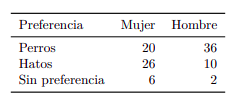
\includegraphics[scale=0.85]{table}
	\end{center}
\end{figure}
\subsection{Encuentra la probabilidad de que un estudiante seleccionado al azar prefiera los perros.}
\paragraph{} Hay un total de 100 estudiantes de los cuales 20 Mujeres y 36 Hombres prefieren a los perros, lo cual significa que 56 de 100 estudiantes prefiere a los perros.\\
Por lo tanto seleccionando al azar a un estudiante habrá $0.56$ de probabilidad que prefiera a los perros. 
\subsection{De acuerdo a los datos obtenidos, ¿los eventos de preferir los perros y ser mujer son mutuamente excluyentes?}
No, pues de serlo significaría que ser mujer implicaría que no prefiera a los perros, sin embargo hay datos de que hay mujeres quienes prefieren a los perros.
\section{Ejercicio 9}
Un estudiante debe elegir una de las siguientes materias: Matemáticas, Física o Química. Es
igualmente probable que elija Matemáticas o Física y doblemente probable que elija Química.
Calcula las probabilidades de cada materia.
\paragraph{Solución: } Sea $x$ la probabilidad de que elija Matemáticas, y que por consiguiente será igual a la probabilidad que elija Física. Tomemos la siguiente ecuación para modelar el problema:
\begin{equation}
	\begin{split}
		1 &= (x + x + 2x)\\
		1 &= 4x\\
		\frac{1}{4} &= x\\
	\end{split}
\end{equation}
Obtenido el valor de $x$ podemos ahora saber las probabilidades de las materias.\\
De que elija Matemáticas $ = 0.25$\\
De que elija Física $ = 0.25$\\
De que elija Química $ = 0.50$\\
\section{Ejercicio 10}
En un concurso de TV el anfitrión le da a un concursante 3 puertas a elegir. Detrás de 2 de
estas puertas hay una cabra y en la restante un auto. El concursante elige la puerta 1 y el
anfitrión descubre la puerta 3, en la cual hay una cabra. Después de descubrir la puerta 2 el
anfitrión le da la opción al concursante de cambiar la puerta 1 que había elegido originalmente
por la puerta 2 aún sin descubrir. ¿Existe alguna diferencia si el concursante cambia de puerta
2? Explica tu respuesta.
\paragraph{} Si, la probabilidad de que el concursante haya escogido la puerta correcta es de $1/3$, dejando $2/3$ en las otras dos puertas.\\ Ahora al eliminar una puerta esas probabilidades se mantienen, concursante sigue con $1/3$ de probabilidad de haber acertado, y también hay $2/3$ en el resto de las puertas, que en este caso ahora solo es una.\\
Finalmente si el concursante cambia de puerta si existe una diferencia, ahora es mas probable que gane.\\
Otro ejemplo sería que en vez de 3 puertas fueran 100, el concursante escoge una puerta y tiene una probabilidad de $1/100$ de escoger la puerta con el auto, si ahora el anfitrión descubre 98 de las 99 puertas restantes, todas con cabras, y le vuelve a dar la opción de cambiar, es mas intuitivo en este caso pensar que si hay diferencia pues la probabilidad de que haya un auto en la puerta que escogió al principio sigue siendo $1/100$ pero la puerta que sobró ahora tiene una probabilidad de $99/100$ de que contenga el auto.
\section{Ejercicio 11}
Calcula la probabilidad de que en un cuarto de 10 personas, al menos 2 cumplan años el
mismo día. Repite el cálculo para 23, 50 y 75 personas y discute los resultados.
\paragraph{Solución: } Sea $E_n$ el evento de que la $n-$ésima persona comparta un cumpleaños con las otras $n-1$ personas.\\
Así lo que buscamos es la probabilidad de que suceda dicho evento para alguna persona $1\leq i \leq n$ donde para el primer ejemplo $n=10$.\\
Ahora revisemos la siguiente ecuación.
\begin{equation}
\begin{split}
1 &= P(E_n) + P(\overline{E_n})\\
1 - P(\overline{E_n}) &= P(E_n)\\
P(E_n) &= 1 - P(\overline{E_n})\\
\end{split}
\end{equation}
Lo que quiere decir que podemos encontrar la probabilidad que buscamos al encontrar la probabilidad del complemento.\\
Entonces el evento $\overline{E_i}$ es que la persona $i$ para $1\leq i\leq n$ con el primer ejemplo de $n=10$ no comparta cumpleaños con alguna otra persona $1 \leq j \leq n$ y $j\neq i$.\\
Veamos como luce la probabilidad de que ninguna persona comparta cumpleaños.\\
\begin{equation}\label{ec11_1}
	\begin{split}
	P(\overline{E_1}\cap \overline{E_2} \cap \dots \cap \overline{E_n}) &=\\
	& \text{al ser eventos independientes}\dots \\
	&= P(\overline{E_1}) \times P(\overline{E_2}) \times \dots \times P(\overline{E_n})
	\end{split}
\end{equation}
Para $i=1$ la probabilidad es 1, pues no hay otra persona con la cual compartir. Supongamos que el año tiene 365 días, ahora para la siguiente persona si no comparte cumpleaños tiene 364 opciones de las 365, pues habrá uno en el comparta con la primera persona. Generalizando tomemos la siguiente ecuación:
\begin{equation}
	\begin{split}
	P(\overline{E_1})=&\frac{365}{365}\\
	P(\overline{E_2})=&\frac{364}{365}\\
	P(\overline{E_3})=&\frac{363}{365}\\
	&\dots\\
	P(\overline{E_i})=&\frac{366 - i}{365}\\
	& \text{para 1 $\leq i \leq n$}\\
	& \text{y para el ejercicio $n \in \{10,23,50,75\}$}\\
	\end{split}
\end{equation}
Ahora sustituyendo en la ecuación \ref{ec11_1}.\\
\begin{equation}\label{ec11_2}
\begin{split}
P(\overline{E_1}) \times P(\overline{E_2}) \times \dots \times P(\overline{E_n}) &=(\frac{365}{365}) \times (\frac{364}{365}) \times (\frac{363}{365}) \times \dots \times (\frac{366 - n}{365}) \\
&=(\frac{1}{365^{n}})\times(365 \times 364 \times 363 \times \dots \times (366 - n))\\
&=(\frac{1}{365^{n}})\times(\frac{365!}{(365-n)!})\\
&=\frac{365!}{365^{n} \times(365-n)!}\\
\end{split}
\end{equation}
Como buscamos el complemento entonces llegamos a la siguiente ecuación:
\begin{equation}\label{ec11_3}
\begin{split}
P(\text{al menos dos personas que compartan cumpleaños})&=1 - \frac{365!}{365^{n} \times(365-n)!}\\
\end{split}
\end{equation}
Sustituyamos ahora $n=10$.
\begin{equation}\label{ec11_4}
\begin{split}
1 - \frac{365!}{365^{n} \times(365-n)!}&=1 - \frac{365!}{365^{10} \times(365-10)!}\\
&\approx 0.117 \\
&\approx 11.7\%
\end{split}
\end{equation}
Para $n=23$.
\begin{equation}
\begin{split}
1 - \frac{365!}{365^{n} \times(365-n)!}&=1 - \frac{365!}{365^{23} \times(365-23)!}\\
&\approx 0.507 \\
&\approx 50.7\%
\end{split}
\end{equation}
Para $n=50$.
\begin{equation}
\begin{split}
1 - \frac{365!}{365^{n} \times(365-n)!}&=1 - \frac{365!}{365^{50} \times(365-50)!}\\
&\approx 0.97 \\
&\approx 97\%
\end{split}
\end{equation}
Para $n=75$.
\begin{equation}
\begin{split}
1 - \frac{365!}{365^{n} \times(365-n)!}&=1 - \frac{365!}{365^{75} \times(365-75)!}\\
&\approx 0.9997 \\
&\approx 99.97\%
\end{split}
\end{equation}
\paragraph{Discusión de resultados:} Los resultados muestran que la probabilidad esta cerca de duplicarse cuando se duplica la $n$, eventualmente llegará a 1 cuando $n=365$, finalmente podemos decir que presenta un comportamiento exponencial.
\section{Ejercicio 12}
Se tiran 2 dados y se registra el número máximo, ¿cuales son las probabilidades de los eventos
1, 2, 3, 4, 5, 6?
\paragraph{Solución: } 
El problema puede modelarse como una combinatoria de $k$ elementos con repetición, en este caso estamos eligiendo 2 elementos de 6 totales. Esto se puede modelar como:

\begin{equation}
	\begin{split}
	\left(\!\!{n\choose k}\!\!\right)&\\
	{n + k - 1 \choose k}&=\\
	&= {6 + 2 - 1 \choose 2} \\
	&= {7 \choose 2} \\
	&= \frac{7!}{2!(7-2)!} \\
	&= \frac{7\times 6 \times 5!}{2!5!} \\
	&= \frac{7\times 6}{2!} \\
	&= \frac{42}{2} \\
	&= 21
	\end{split}
\end{equation}
Entonces al tirar dos dados existen 21 posibles resultados.\\
De los cuales entonces hay que revisar los casos donde el numero 6 es el mayor. Son $\{(1,6), (2,6), (3, 6), (4, 6), (5, 6), (6, 6)\}$. Son 6 de los posibles 21 casos. Por lo tanto la probabilidad de que $6$ sea el número mayor al tirar 2 dados es de $\frac{6}{21} = \frac{2}{7} = 0.2857$.\\
Donde el numero 5 es el mayor. Son $\{(1,5), (2,5), (3, 5), (4, 5), (5, 5)\}$. Son 5 de los posibles 21 casos. Por lo tanto la probabilidad de que $5$ sea el número mayor al tirar 2 dados es de $\frac{5}{21} = 0.2381$.\\
Donde el numero 4 es el mayor. Son $\{(1,4), (2,4), (3, 4), (4, 4)\}$. Son 4 de los posibles 21 casos. Por lo tanto la probabilidad de que $4$ sea el número mayor al tirar 2 dados es de $\frac{4}{21} = 0.19047$.\\
Donde el numero 3 es el mayor. Son $\{(1,3), (2,3), (3, 3)\}$. Son 3 de los posibles 21 casos. Por lo tanto la probabilidad de que $3$ sea el número mayor al tirar 2 dados es de $\frac{3}{21} = \frac{1}{7} = 0.14285$.\\
Donde el numero 2 es el mayor. Son $\{(1,2), (2,2)\}$. Son 2 de los posibles 21 casos. Por lo tanto la probabilidad de que $2$ sea el número mayor al tirar 2 dados es de $\frac{2}{21} = 0.095238$.\\
Donde el numero 1 es el mayor. Son $\{(1,1)\}$. Son 1 de los posibles 21 casos. Por lo tanto la probabilidad de que $1$ sea el número mayor al tirar 1 dados es de $\frac{1}{21} = 0.047619$.\\
\section{Ejercicio 13}
 Prueba que la covarianza de 2 variables independientes es 0.
\paragraph{Solución: } La covarianza esta definida como:
\begin{equation}\label{e13_1}
	cov(X,Y)=E[XY] - E[X]E[Y]
\end{equation} 
Si queremos probar que la covarianza es cero debemos probar que se cumple la siguiente igualdad:
\begin{equation}
\begin{split}
cov(X,Y)&=E[XY] - E[X]E[Y]\\
0&=E[XY] - E[X]E[Y]\\
E[X]E[Y]&=E[XY]\\
\end{split}
\end{equation}
Tomemos la definición del valor esperado para el producto de dos variables:
\begin{equation}
	E[XY] = \int \int xyF_{X,Y}(x,y)dxdy 
\end{equation}
Ahora al ser independientes la función de probabilidad para que ambas variables se puede descomponer en un producto de 2 funciones. 
\begin{equation}
\begin{split}
E[XY] &= \int \int xyF_{X,Y}(x,y)dxdy\\
&= \int \int xyF_{X}(x)F_{Y}(y)dxdy\\
\end{split}
\end{equation}
Posteriormente reagrupamos las integrales:
\begin{equation}
\begin{split}
E[XY] &= \int \int xyF_{X}(x)F_{Y}(y)dxdy\\
&= \int xF_{X}(x)dx \int yF_{Y}(y)dy\\
\end{split}
\end{equation}
Cada integral pasa a describir el valor esperado de X y de Y.
\begin{equation}
\begin{split}
E[XY] &= \int xF_{X}(x)dx \int yF_{Y}(y)dy\\
&= E[X]E[Y]\\
\end{split}
\end{equation}
La cual era la igualdad a la que queríamos llegar entonces al ser iguales podemos tomar la ecuación \ref{e13_1} y sustituir:
\begin{equation}
\begin{split}
cov(X,Y)&=E[XY] - E[X]E[Y]\\
&= E[X]E[Y] - E[X]E[Y]\\
&= 0\\
\end{split}
\end{equation}
Finalmente llegamos a que la covarianza de dos variables independientes es 0.
\section{Ejercicio 14}
 Un alumno decide responder de forma aleatoria un examen en el que cada pregunta tiene
5 opciones de las cuales solo 1 es correcta. Suponiendo que la probabilidad de acertar una
pregunta es de 0.2 y que cada respuesta es independiente de las demás, calcula lo siguiente:\\
\subsection{La probabilidad de tener 10, 20 y 40 aciertos si el examen consiste de 50 preguntas}
El problema plantea calcular la probabilidad de un numero de éxitos en una serie de "experimentos" los cuales son cada pregunta del examen, tomando que los eventos son independientes y que hay una probabilidad definida de éxito $p=0.2$ para cada uno podemos entonces modelar una distribución binomial:
\begin{equation}
\begin{split}
b(x;n;p)={n\choose x} \times p^x \times (1 - p)^{n-x}
\end{split} 
\end{equation}
Así entonces podemos encontrar la probabilidad con $x \in \{10, 20, 40\}$ para $n=50$.\\
Para $x=10$:\\
\begin{equation}
\begin{split}
b(10;50;0.2)&={50\choose 10} \times 0.2^{10} \times (1 - 0.2)^{50-10}\\
&=(\frac{50!}{10!\times(50-10)!}) \times 0.2^{10} \times 0.8^{40}\\
&=(\frac{50!}{10!\times(40)!}) \times 0.2^{10} \times 0.8^{40}\\
&=(\frac{50!}{10!\times(40)!}) \times 0.2^{10} \times 0.8^{40}\\
&= 0.13981900517
\end{split} 
\end{equation}
Para $x=20$:\\
\begin{equation}
\begin{split}
b(20;50;0.2)&={50\choose 20} \times 0.2^{20} \times (1 - 0.2)^{50-20}\\
&=(\frac{50!}{20!\times(50-20)!}) \times 0.2^{20} \times 0.8^{30}\\
&=(\frac{50!}{20!\times(30)!}) \times 0.2^{20} \times 0.8^{30}\\
&=(\frac{50!}{20!\times(30)!}) \times 0.2^{20} \times 0.8^{30}\\
&= 0.00061177215
\end{split} 
\end{equation}
Para $x=40$:\\
\begin{equation}
\begin{split}
b(40;50;0.2)&={50\choose 40} \times 0.2^{40} \times (1 - 0.2)^{50-40}\\
&=(\frac{50!}{40!\times(50-40)!}) \times 0.2^{40} \times 0.8^{10}\\
&=(\frac{50!}{40!\times(10)!}) \times 0.2^{40} \times 0.8^{10}\\
&=(\frac{50!}{40!\times(10)!}) \times 0.2^{40} \times 0.8^{10}\\
&\approx 1.2 \times 10^{-19}
\end{split} 
\end{equation}
\subsection{La probabilidad de tener 10, 20 y 40 aciertos si el examen consiste de 40 preguntas}
Para $x=10$:\\
\begin{equation}
\begin{split}
b(10;40;0.2)&={40\choose 10} \times 0.2^{10} \times (1 - 0.2)^{40-10}\\
&=(\frac{40!}{10!\times(40-10)!}) \times 0.2^{10} \times 0.8^{30}\\
&=(\frac{40!}{10!\times(30)!}) \times 0.2^{10} \times 0.8^{30}\\
&=(\frac{40!}{10!\times(30)!}) \times 0.2^{10} \times 0.8^{30}\\
&= 0.10745373771
\end{split} 
\end{equation}
Para $x=20$:\\
\begin{equation}
\begin{split}
b(20;40;0.2)&={40\choose 20} \times 0.2^{20} \times (1 - 0.2)^{40-20}\\
&=(\frac{40!}{20!\times(40-20)!}) \times 0.2^{20} \times 0.8^{20}\\
&=(\frac{40!}{20!\times(20)!}) \times 0.2^{20} \times 0.8^{20}\\
&=(\frac{40!}{20!\times(20)!}) \times 0.2^{20} \times 0.8^{20}\\
&= 0.00001666462
\end{split} 
\end{equation}
Para $x=40$:\\
\begin{equation}
\begin{split}
b(20;40;0.2)&={40\choose 40} \times 0.2^{40} \times (1 - 0.2)^{40-40}\\
&=(\frac{40!}{40!\times(40-40)!}) \times 0.2^{40} \times 0.8^{0}\\
&=(\frac{40!}{40!\times(0)!}) \times 0.2^{40} \\
&=(\frac{40!}{40!}) \times 0.2^{40} \\
&= 0.2^{40} \\
&\approx 1.1 \times 10^{-26}
\end{split} 
\end{equation}
\subsection{La probabilidad de tener 10, 20 y 40 errores si el examen consiste de 40 preguntas}
Para 10 errores significan 30 aciertos, es decir $x=30$:\\
\begin{equation}
\begin{split}
b(30;40;0.2)&={40\choose 30} \times 0.2^{30} \times (1 - 0.2)^{40-30}\\
&=(\frac{40!}{30!\times(40-30)!}) \times 0.2^{30} \times 0.8^{10}\\
&=(\frac{40!}{30!\times(10)!}) \times 0.2^{30} \times 0.8^{10}\\
&=(\frac{40!}{30!\times(10)!}) \times 0.2^{30} \times 0.8^{10}\\
&\approx 9 \times 10^{-14}
\end{split} 
\end{equation}
Para 20 errores significan 20 aciertos, es decir $x=20$:\\
\begin{equation}
\begin{split}
b(20;40;0.2)&={40\choose 20} \times 0.2^{20} \times (1 - 0.2)^{40-20}\\
&=(\frac{40!}{20!\times(40-20)!}) \times 0.2^{20} \times 0.8^{20}\\
&=(\frac{40!}{20!\times(20)!}) \times 0.2^{20} \times 0.8^{20}\\
&=(\frac{40!}{20!\times(20)!}) \times 0.2^{20} \times 0.8^{20}\\
&= 0.00001666462
\end{split} 
\end{equation}
Para 40 errores significan 0 aciertos, es decir $x=0$:\\
\begin{equation}
\begin{split}
b(0;40;0.2)&={40\choose 0} \times 0.2^{0} \times (1 - 0.2)^{40-0}\\
&=(\frac{40!}{0!\times(40-0)!}) \times 0.8^{40}\\
&=(\frac{40!}{40!}) \times 0.8^{40}\\
&= 0.8^{40}\\
&= 0.0001329228
\end{split} 
\end{equation}
\section{Ejercicio 15}
La estatura promedio de los alumnos de una universidad es de 169.83cm, con una desviación
estándar de 4.5cm. Suponiendo una distribución normal, calcula la probabilidad de que la
estatura de un alumno dado:
\subsection{Se encuentre entre 160cm y 180cm}
\subsection{Sea de al menos 150cm}
\subsection{Sea de máximo 180cm}
\subsection{Sea mayor a 160cm}
\subsection{Sea menor a 190cm}
\section{Ejercicio 16}
Se tiene la siguiente información acerca del clima. La probabilidad de que llueva el día de hoy
es de 0.6, mientras que la probabilidad de que llueva el día de mañana es de 0.5. Además, se
sabe que la probabilidad de que ningún día llueva es de 0.3. Considerando dicha información
encuentre las siguientes probabilidades:
\subsection{Que llueva hoy o mañana.}
Sea H el evento de que llueva hoy, y sea M el evento de que llueva mañana.\\
En la descripción del problema tenemos que la probabilidad de que ningún día llueva es de 0.3. Es decir:
\begin{equation}
	P(\overline{H} \cap \overline{M}) = 0.3
\end{equation}
Lo que estamos buscando es lo inverso, es decir:
\begin{equation}
\begin{split}
P(\overline{\overline{H} \cap \overline{M}}) &= 1 - 0.3 \\
P(\overline{\overline{H} \cap \overline{M}}) &= 0.7 \\
P(H \cup M) &= 0.7 \\
\end{split}
\end{equation}
Finalmente tenemos que la probabilidad de H o M es de 0.7.
\subsection{Que llueva hoy y mañana.}
Podemos tomar la siguiente ecuación con la que se calcula la probabilidad de que llueva hoy (H) o que llueva mañana (M).\\
\begin{equation}\label{ec16_1}
	\begin{split}
		P(H\cup M) &= P(H) + P(M) - P(H\cap M)\\
		P(H\cup M) + P(H\cap M) &= P(H) + P(M)\\
		P(H\cap M) &= P(H) + P(M) - P(H\cup M)\\
	\end{split}
\end{equation}
Ahora como contamos con la probabilidad de H y de M por la descripción del problema y tenemos $P(H\cup M)$ por el punto anterior podemos sustituir dichos valores en la ecuación \ref{ec16_1}.
\begin{equation}\label{ec16_2}
\begin{split}
P(H\cap M) &= 0.6 + 0.5 - 0.7\\
&= 0.4\\
\end{split}
\end{equation}
Finalmente decimos que la probabilidad de que llueva hoy y mañana es de $0.4$.
\subsection{Que llueva hoy pero no mañana.}
Lo que buscamos es $P(H\backslash (H\cap M))$.
\begin{equation}\label{ec16_3}
\begin{split}
P(H\backslash (H\cap M)) &= P(H) - P(H\cap M)\\
&= 0.6 - 0.4\\
&= 0.2\\
\end{split}
\end{equation}
Finalmente decimos que la probabilidad de que llueva hoy pero no mañana es de $0.2$.
\subsection{Que llueva hoy o mañana, pero no ambas.}
Lo que buscamos es la diferencia simétrica la cual podemos expresar como:
\begin{equation}\label{ec16_5}
\begin{split}
P(H\triangle M) &= P((H\cup M) \backslash (H\cap M))\\
&= P(H\cup M) - P(H\cap M)\\
\end{split}
\end{equation}
Y ambos valores en la ecuación \ref{ec16_5} los tenemos así solo sustituimos.
\begin{equation}\label{ec16_6}
\begin{split}
P(H\triangle M) &= P(H\cup M) - P(H\cap M)\\
&= 0.7 - 0.4\\
&= 0.3\\
\end{split}
\end{equation}
Finalmente decimos que la probabilidad de que llueva hoy o mañana pero no ambas es de $0.3$. 
\section{Ejercicio 17}
Una empresa de lámparas incandecentes observa que el número de componentes que fallan
antes de cumplir 100 horas de funcionamiento es una variable aleatoria de Poisson. Si el
número promedio de estos fallos es 8, calcule lo siguiente:
\subsection{¿Cuál es la probabilidad de que falle 1 componente en 25 horas?}
Si es una variable aleatoria con una distribución de Poisson, la probabilidad de ocurrencia de eventos esta dada por:
\begin{equation}
	\begin{split}
		P(x)=\frac{\lambda^xe^{-\lambda}}{x!}
	\end{split}
\end{equation}
Donde $\lambda$ es el promedio de eventos por intervalo.\\
$e$ es el número de Euler.\\
$x$ es el número de eventos.\\
En nuestro caso $\lambda = 8$ para un intervalo de 100 horas, así el promedio en un intervalo de 25 horas sería $\lambda=2$.\\
\begin{equation}
	\begin{split}
	P(1) &= \frac{2^1e^{-2}}{1!}\\
	&= \frac{2e^{-2}}{1}\\
	&= 2e^{-2}\\
	&\approx 0.2711\\
	\end{split}
\end{equation}
\subsection{¿Cuál es la probabilidad de que fallen no más de 2 componentes en 50 horas?}
Ahora $\lambda=4$ y la probabilidad puede verse como la suma de que no fallen, falle 1 y fallen 2.\\
\begin{equation}
\begin{split}
P(x\leq2)&= \sum_{n=0}^{2} \frac{4^ne^{-4}}{n!}\\
 &= \frac{4^0e^{-4}}{0!} + \frac{4^1e^{-4}}{1!} + \frac{4^2e^{-4}}{2!}\\
&= \frac{1 e^{-4}}{1} + \frac{4e^{-4}}{1} + \frac{4^2e^{-4}}{2}\\
&= e^{-4} + 4e^{-4} + 8e^{-4}\\
&\approx 0.238\\
\end{split}
\end{equation}
\subsection{¿Cuál es la probabilidad de que fallen por lo menos 10 en 125 horas?}
Ahora $\lambda=10$ y la probabilidad puede verse como la suma de que no fallen hasta 9 y sacar el complemento.\\
\begin{equation}
\begin{split}
P(x\geq10)&= 1 - P(x<10)\\
\end{split}
\end{equation}
\begin{equation}
\begin{split}
P(x<10)&= \sum_{n=0}^{9} \frac{10^ne^{-10}}{n!}\\
&\approx 0.54207\\
\end{split}
\end{equation}
\section{Ejercicio 18}
 El consejo universitario de la Facultad de Ciencias está compuesto por 14 miembros, 5 de los
cuales son estudiantes, 5 son maestros y 4 son investigadores. Un periodista planea seleccionar
a 2 de los miembros del consejo para realizarles una entrevista. El primer miembro será elegido
al azar y el segundo será elegido al azar de los miembros restantes. ¿Cuál es la probabilidad
de que se seleccionen 2 maestros?
\paragraph{Solución: } Tomemos la probabilidad de que el primer miembro seleccionado al azar resulte ser maestro.\\
En este caso hay 5 maestros en el consejo de 14 miembros, por lo tanto hay una probabilidad de $\frac{5}{14}$ de seleccionar a un maestro.\\
Ahora si queremos dado ese caso seleccionar a otro maestro tendremos 4 maestros en 13 miembros restantes, así que seleccionemos a un segundo maestro tendrá una probabilidad de $\frac{4}{13}$.
Y la probabilidad de que sucedan ambos esta dado por su producto.\\
\begin{equation}
	\begin{split}
	\frac{5}{14} \times \frac{4}{13}&=\\
	&=\frac{5\times 4}{14 \times 13} \\
	&=\frac{20}{182} \\
	&=\frac{10}{91}\\
	&= 0.109890
	\end{split}
\end{equation}
\section{Ejercicio 19}
Una baraja ordinaria de 52 cartas se divide aleatoriamente en 4 pilas de 13 cartas cada una.
Calcule la probabilidad de que cada pila tenga exactamente 1 As.\\
Hay 4 Ases, tomemos el caso para el primer As, este As estará en alguna de las 4 pilas y no tendríamos mayor inconveniente.\\
Ahora para el segundo As requiere forzosamente estar en otra pila que no sea la del segundo, si cada pila tiene 13 cartas, entonces El segundo As debió estar en las 39 cartas restantes que no pertenecen a la primera pila y que no sea el primer as, lo cual tiene una probabilidad de $\frac{39}{51}$.\\
Para el tercer As no debió estar ni en la primera, ni en la segunda pila lo cual significa que debió estar en las 26 cartas restantes y que no son los primeros 2 ases con una probabilidad de $\frac{26}{50}$.\\
Para el último As debió estar en las últimas 13 cartas y que no es alguno de los otros ases con una probabilidad de $\frac{13}{49}$.\\
Finalmente terminar con un As en cada pila significa que todos estos eventos pasaron y podemos encontrar el valor con un producto.
\begin{equation}
\begin{split}
	1 \times \frac{39}{51} \times \frac{26}{50} \times \frac{13}{49} &= 0.1055\\	
\end{split}
\end{equation}
\section{Ejercicio 20}
 En una determinada etapa de una investigación criminal el inspector al mando está 60 \%
convencido de la culpabilidad de un sospechoso. Supongamos, sin embargo, que una nueva
pieza de evidencia muestra que el delincuente tiene una cierta característica (como la calvicie
o el pelo castaño). Si el 20 por ciento de la población posee esta característica, ¿cuál es la
certeza de la culpabilidad del sospechoso que tiene el inspector si resulta que el sospechoso
tiene la característica?\\
\paragraph{Solución:} Sea $C$ el evento de que el individuo sea culpable según la sospecha del detective, entonces $P(C) = 60\% = 0.6$, ahora de que sea inocente ($I$) es $P(C) = 40\% = 0.4$, el evento de que una persona posea la característica la podemos definir como:
$P(C_r) = 20\% = 0.2$.\\
Lo que estamos buscando es la certeza de culpabilidad dado que tiene la característica, es decir:
\begin{equation}
	P(C|C_r)
\end{equation}
Ahora la cual podemos desarrollar con el teorema de Bayes:
\begin{equation}
\begin{split}
P(C|C_r)&=\frac{P(C_r|C)\times P(C)}{P(C_r)}\\
&=\frac{P(C_r|C)\times P(C)}{P(C_r|C)\times P(C) + P(C_r|I)\times P(I)}\\
&=\frac{1\times 0.6}{1\times 0.6 +  0.2 \times 0.4}\\
&= 0.8823529411764707\\
&\approx 88.23\%\\
\end{split}
\end{equation}
\end{document}  